% --*- coding:utf-8-unix mode:latex -*--
%\include{Begin}
%%%%%%%%%%%%%%%%%%%%%%%%%%%%%%%%%%%%%%%%%%%%%%%%%%%%%%%%%%%%%%%%%%%%%%%%%%%%%%%
\section{先遣隊}

\subsection{日時・場所}

\begin{tabular}{p{2zw}rp{38zw}}
  日時 & : & 2019年4月5日(金) 8:30 $\sim$ 15:30\\
  場所 & : & 工科大学 $\sim$ 国立幡多青少年自然の家
\end{tabular}

\subsection{目的}
本隊より先遣し国立幡多青少年自然の家に向かい,本隊が到着後円滑にセミナーが進行できるように事前準備を行う

\subsection{タイムスケジュール}
% 時刻は必ず4桁(00:00)で書くこと!!!
\begin{longtable}{p{3zw}p{39zw}}

  08:30 & \textbf{◎ 出発} \\
        & \ \  ※休憩を取りながら向かう \\\\

  11:00 & \textbf{◎ 到着} \\
        & \ \  \textbullet \ \ 3台とも到着次第,横田が報告slackに連絡する \\\\

  11:10 & \textbf{◎ 打ち合わせ(ロビー)} \\ %部屋の鍵は全て開錠(22:00まで)
        & \ \ \textbullet \ \ 施設の方と最終的な打ち合わせを行い,変更点等があれば報告slackに連絡する \\
        & \ \ \textbullet \ \ 打ち合わせの際,入所式時に来てくださる職員さんに来る時間 (15:30ごろ)を伝える \\
        & \ \ \textbullet \ \ 終了次第,準備を始める \\\\
        
        & \textbf{◎ 物品搬入} \\
        & \ \ \textbullet \ \ 車をロータリーに停めておき,物品をおろす \\
        & \ \ \textbullet \ \ おろした物品は第四研修室に入れる \\
        & \ \ \textbullet \ \ (雨天時)手の空いているスタッフは玄関に置いてある傘立てを研修生入口へ移動させる \\\\

        & \textbf{◎ 第一研修室, 第二研修室,大研修室準備} \\
        & \ \ \textbullet \ \ 第一・二研修室の机を荷物を置けるように配置する(図\ref{fig:nimotsuhaichi}参照) \\
        & \ \ \textbullet \ \ 第四研修室は物品置き場のため机等は出さない \\
        & \ \ \textbullet \ \ 小松,横田,以西は,第一・二研修室の机に,野外炊事班の班名を書いた紙を貼る(図\ref{fig:nimotsuhaichi}参照) \\
        & \ \ \textbullet \ \ 小島,野田,三浦は,イスを大研修室に移動させる \\ %先生の人数分の椅子
        & \ \ \textbullet \ \ 小松,横田,以西は大研修室に移動し,小島,野田,三浦が運んでいたイスを受け取り設置する(図\ref{fig:daikenshuhaichi}参照) \\\\
        
        \newpage

        & \textbf{◎ 大研修室設営,マイク確認} \\
        & \ \ \textbullet \ \ 運ばれているイスを設営 \\
        & \ \ \textbullet \ \ 学年担任の松崎先生は1番左(司会者寄り)にする \\
        & \ \ \textbullet \ \ マイク,音響の確認を行う \\
        & \ \ \textbullet \ \ 野外炊事班を示したプラカードを設置する \\\\

 14:00  & \textbf{◎ シーツ,布団カバー,枕カバーを数える,運搬(小松,横田)} \\
        & \ \ \textbullet \ \ 宿泊する人数分を数える \\
        & \ \ \textbullet \ \ 各棟に分ける \\
        	\hspace{15mm} & \ \ \ \ \ ※ \ \ \ 女性教職員:\ 1部屋(7人+子供) \\
        	\hspace{15mm} & \ \ \ \ \ ※ 女性スタッフ:\ 2部屋(11人) \\
        	\hspace{15mm} & \ \ \ \ \ ※ \ \ \ 新入生女子:\ 3部屋(24人) \\
        	\hspace{15mm} & \ \ \ \ \ ※ \ \ \ 新入生男子:11部屋(90人) \\
        	\hspace{15mm} & \ \ \ \ \ ※ 男性スタッフ:\ 4部屋(24人) \\
        	\hspace{15mm} & \ \ \ \ \ ※ \ \ \ 男性教職員:\ 3部屋(18人) \\
        & \ \ \textbullet \ \ 数えたシーツ,布団カバー,枕カバーを各部屋に運搬する
        		(図\ref{fig:seatshaichi},\ref{fig:shushin}参照) \\\\

        & \textbf{◎ ドライヤーの設置(三浦,以西)} \\
        & \ \ \textbullet \ \ 洗面台にドライヤー2つずつとミーティングルーム横の洗面台にヘアアイロン1つ(男子用),
        		新入生女子・男子部屋のいずれか2部屋にドライヤーを1つずつ設置する(図\ref{fig:shushin}参照) \\
        & \ \ \textbullet \ \ 他のヘアアイロンは女性スタッフの部屋にすべて置いておく \\\\

        & \textbf{◎ 野外炊事場準備(小島,野田)}  \\
        & \ \ \textbullet \ \ 机を9.6, 9.7を元に配置する \\
        & \ \ \textbullet \ \ 机に野外炊事班の班名を書いた紙を貼る \\
        & \ \ \textbullet \ \ 入所式には全員が参加する必要があるため,準備を終えたら帰ってくる \\
        & \ \ \textbullet \ \ 間に合わないときは宮尾に連絡し,準備を続ける \\\\

 14:30   & \textbf{◎ 事務室前集合(小島,小松,横田,野田,以西,三浦)} \\
         & \ \ \textbullet \ \ 事務室に集合し,次の動きに備える \\
         & \ \ \textbullet \ \ 雨天時:以西,三浦が荷物を置くためのブルーシートを玄関前に広げる \\\\

 15:00   & \textbf{◎ 新入生の誘導(小島,小松,横田,野田,以西,三浦)} \\
         & \ \ \textbullet \ \ それぞれが誘導場所に待機し準備をする(図\ref{fig:hare}参照) \\
         %& \ \ \textbullet \ \ 残りの人は入所式を行う大研修室に向かう \\
         & \ \ \textbullet \ \ 研修生入口まではバス内のスタッフが誘導する \\
         & \ \ \textbullet \ \ 全ての準備が終了し,手が空いていた場合は全員で誘導する \\
         & \ \ \textbullet \ \ 人手が足りない場合は横田,以西,小松,三浦のみ誘導する \\
         & \ \ \ \ \ 1. 小島:玄関前 \\
         & \ \ \ \ \ 2. 横田:入り口前 \\
         & \ \ \ \ \ 3. 野田:ロビー \\
         & \ \ \ \ \ 4. 以西:第一研修室前 \\
         & \ \ \ \ \ 5. 小松:第二研修室前 \\
         & \ \ \ \ \ 6. 三浦:大研修室内 \\\\

\end{longtable}

\newpage

\subsection{人員配置(人数により調整,運転者含む)}
\begin{itemize}
\item 先遣隊1:小島(車),宮尾
\item 先遣隊2:小松(車), 横田
\item 先遣隊3:三浦(車),野田,以西
\end{itemize}

\subsection{配置図}

\subsubsection{荷物の配置}

\begin{figure}[htbp]
 \begin{center}
  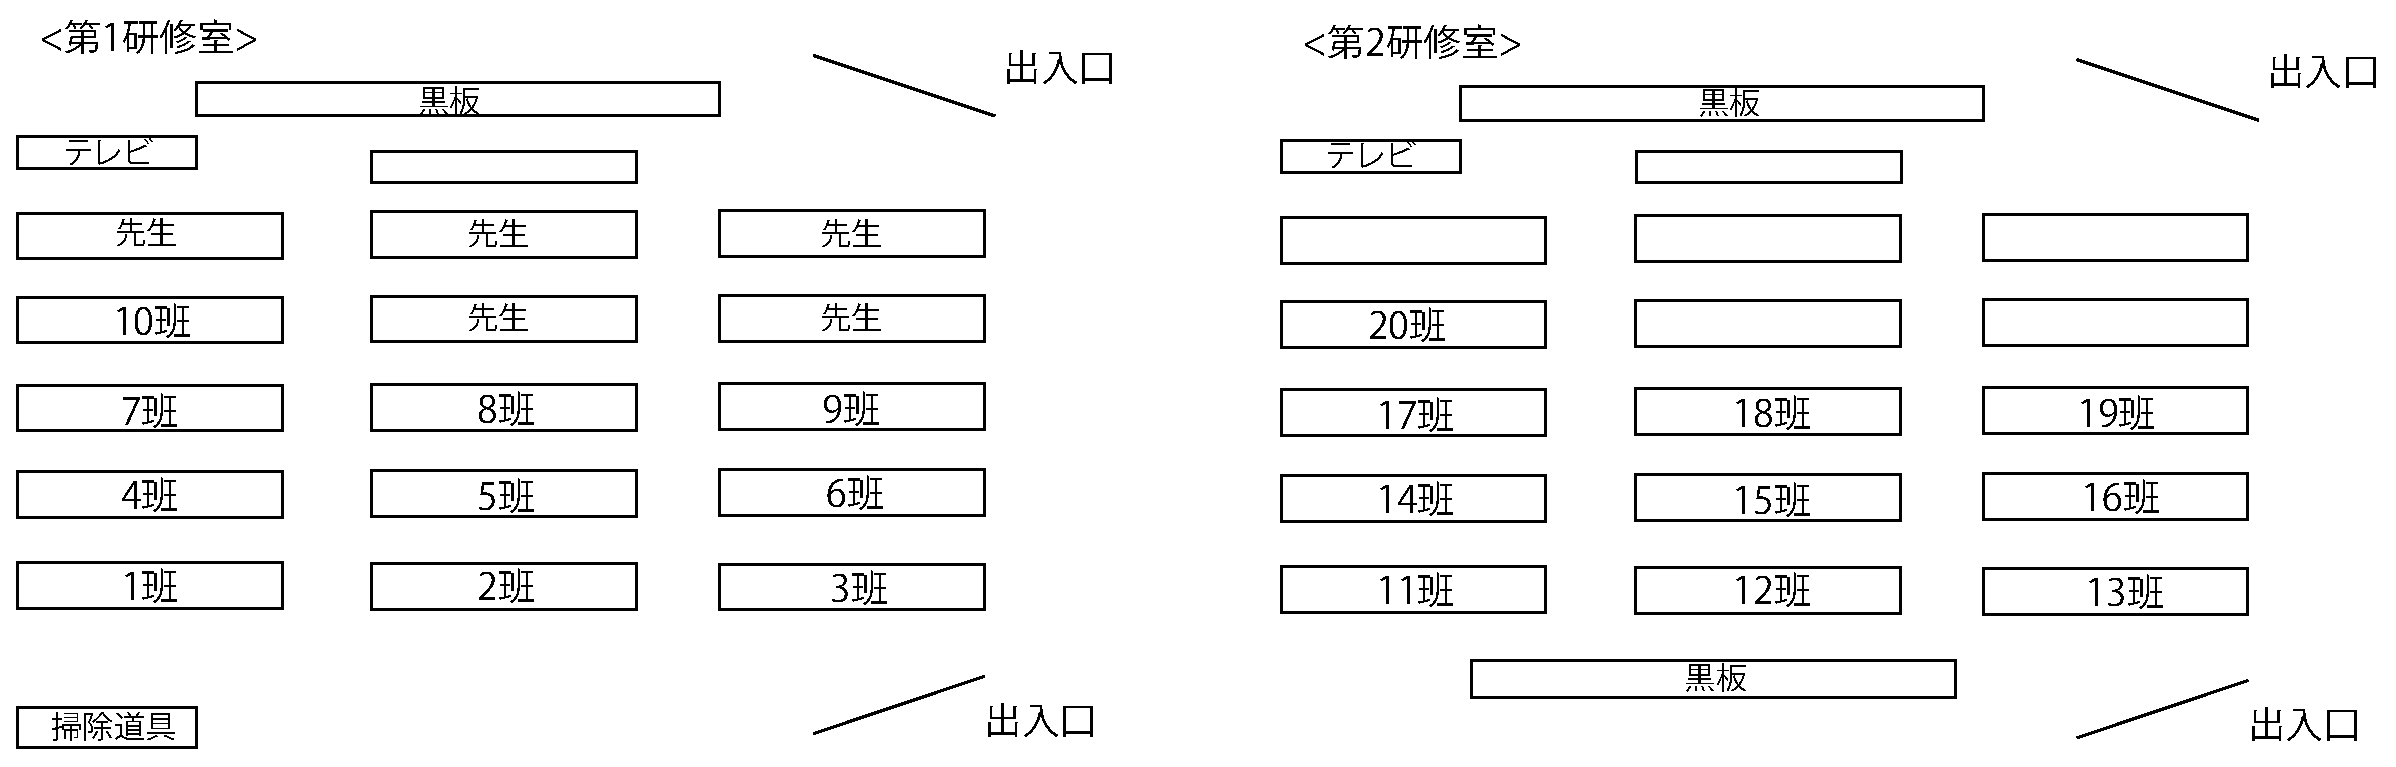
\includegraphics[width=150mm]{./03/nimotsu.eps}
\end{center}
 \caption{第一・二研修室での荷物を置く配置}
 \label{fig:nimotsuhaichi}
\end{figure}
\vspace{-10mm}
\subsubsection{シーツ置き場}

\vspace{-30mm}

\begin{figure}[H]
 \begin{center}
 \hspace{-20mm}
  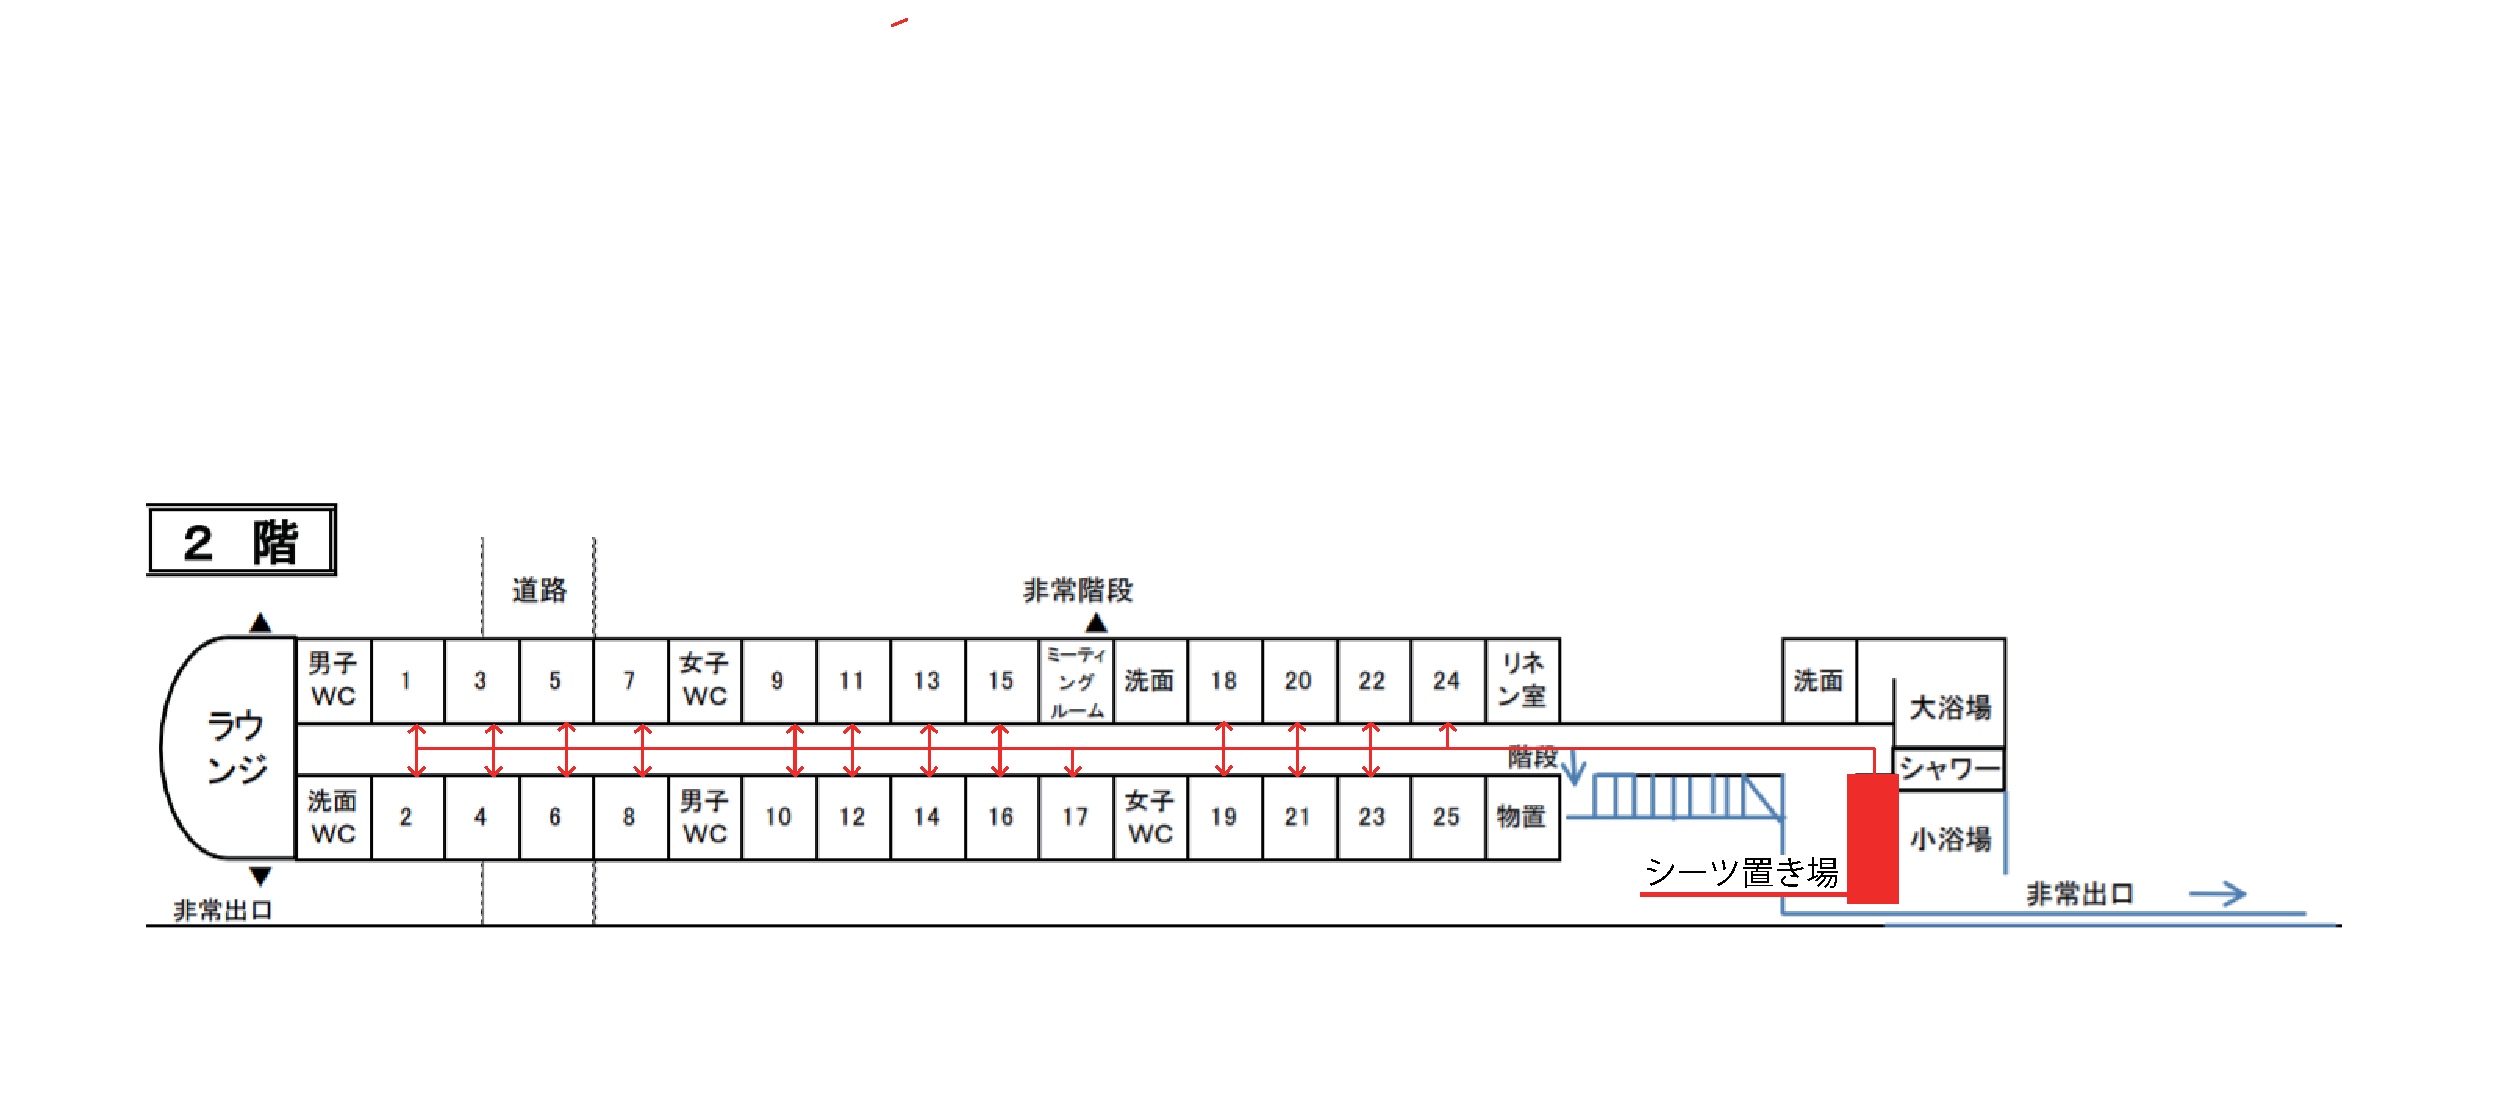
\includegraphics[width=180mm,scale=0.45]{./03/situ.eps}
\end{center}
\vspace{-15mm}
 \caption{シーツを置く位置}
 \label{fig:seatshaichi}
\end{figure}

\subsection{就寝部屋割り}
\begin{figure}[H]
\begin{center}
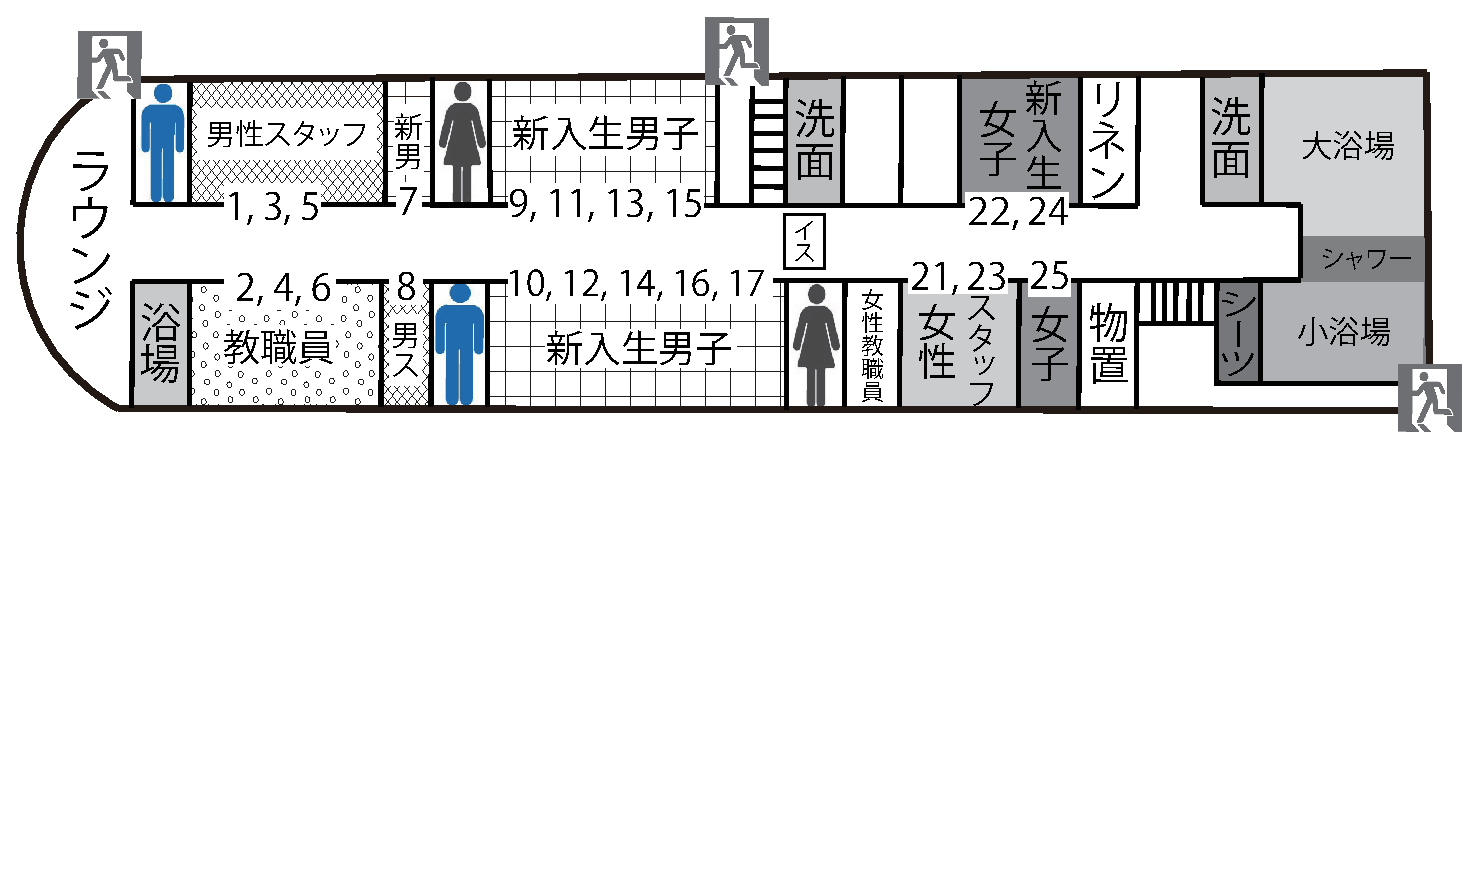
\includegraphics[scale=0.5]{./10/syushin.eps}
\vspace{-30mm}
\caption{就寝部屋}
\label{fig:shushin}
\end{center}
\end{figure}

\subsubsection{大研修室の配置}
\begin{figure}[H]
 \begin{center}
  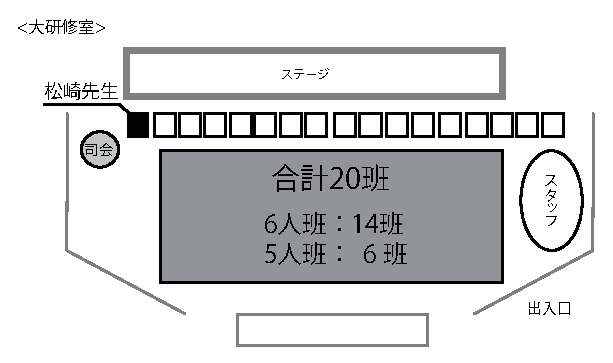
\includegraphics[width=130mm]{./03/nyushoshiki.eps}
  \end{center}
 \caption{大研修室の配置}
 \label{fig:daikenshuhaichi}
\end{figure}

\subsubsection{大研修室誘導時の配置}
\begin{figure}[htbp]
  \begin{center}
   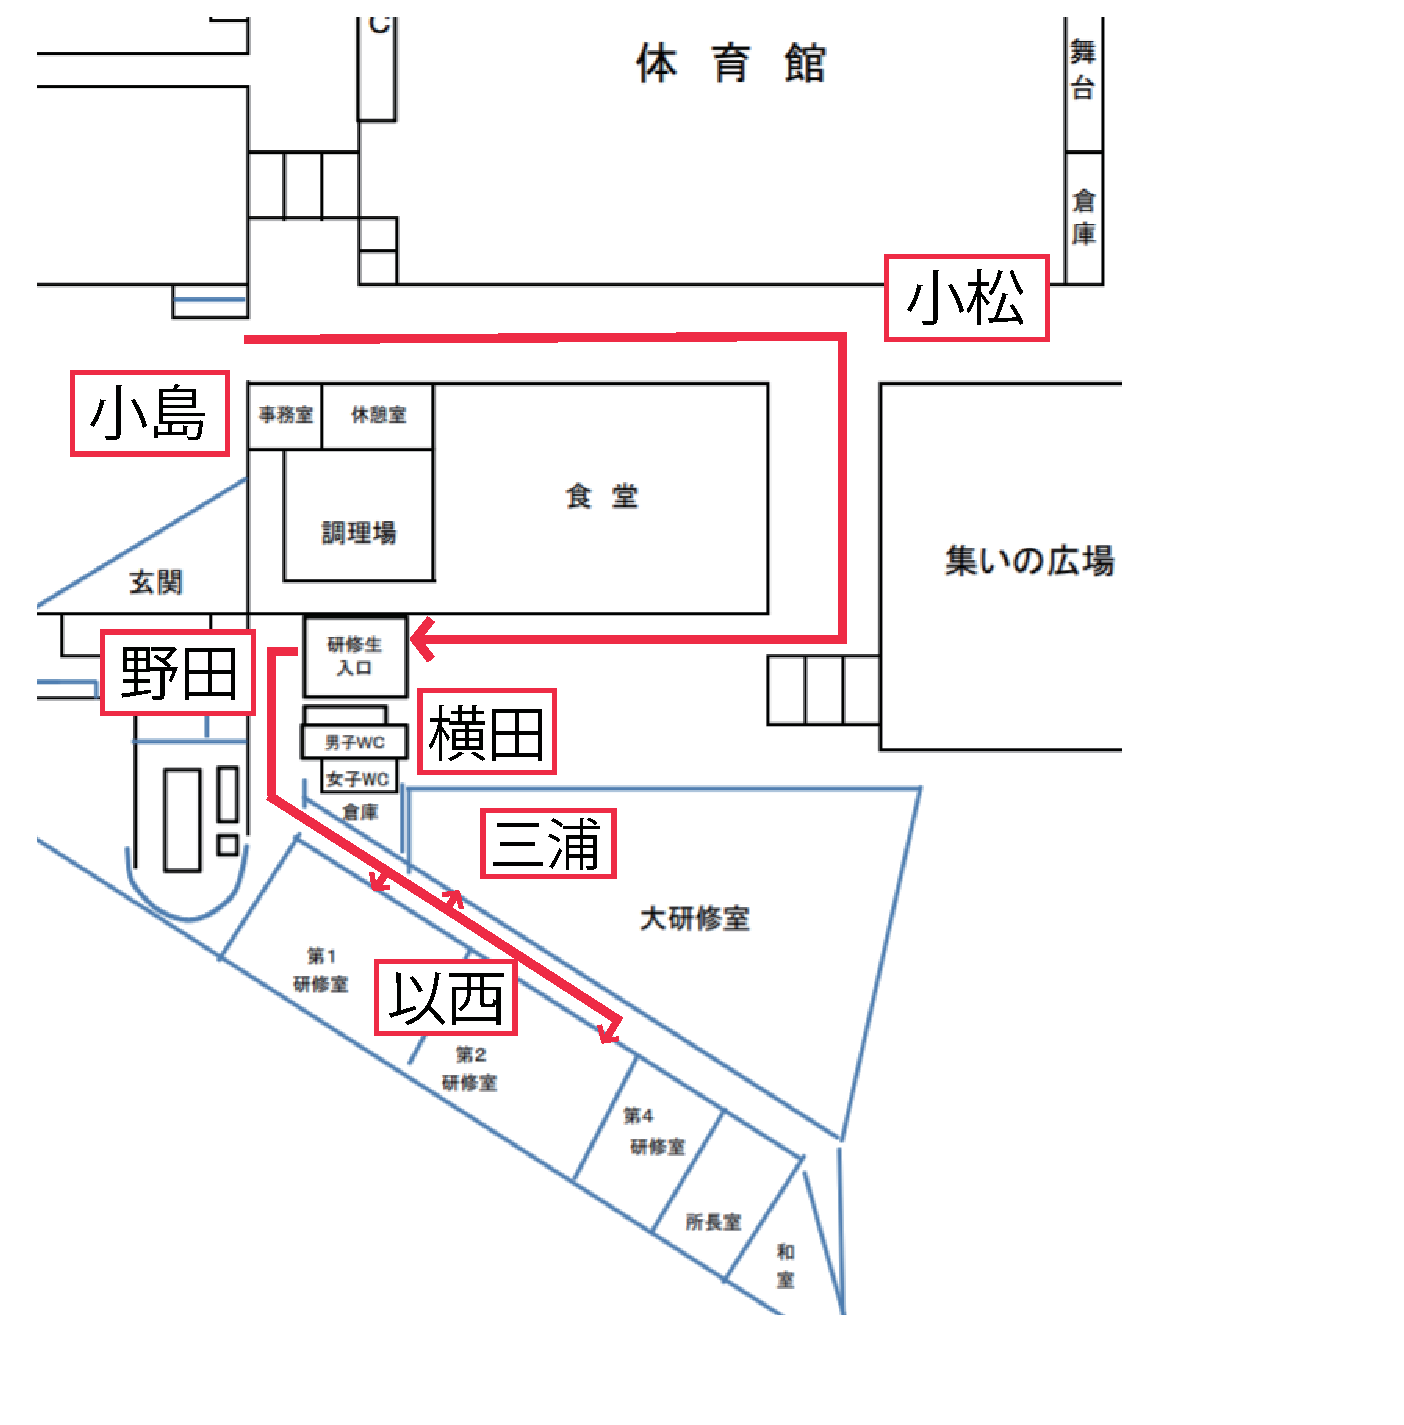
\includegraphics[scale=0.4]{./03/yuudou.eps}
  \end{center}
  \caption{大研修室までの誘導}
  \label{fig:hare}
\end{figure}

\newpage

\subsection{必要物品}
\begin{itemize}
\item 大研修室用の野外炊事班を示したプラカード:20枚
\item 第一・二研修室用の野外炊事班を示した用紙:20枚
\item 野外炊事場用の野外炊事班を示した用紙:20枚
\item 教員名を印刷した紙:25枚
\item マスキングテープ(イスに教職員名を貼り付ける用):1つ
\item ブルーシート:2つ(清水研究室)
\item プロジェクタ:3つ(2つは学校,1つは幡多青少年自然の家)
\item スクリーン:1つ(清水研究室)
\item マイク(幡多)
\item 椅子(先生用)
\item 野外炊事物品:食器用消毒液(20+1(引き継ぎ)),ふきん(24枚),予備の着火剤(2),予備のチャッカマン(2),予備のうちわ(10),予備のポリ袋(20)
\end{itemize}

\subsection{備考}
\begin{itemize}
\item バスの所在を随時連絡してもらうので時間を考えて行動する
\item 先遣隊で連絡を取り合い,終わっていないところの救援を行う
\item マイクの電池を確認しておく
\item 入所式に班名が書かれたプラカードを設置する
\item 部屋の鍵は全て開錠されている(22:00に施錠される)
\end{itemize}

\subsection{連絡事項}
\begin{table}[h]
\begin{center}
\begin{tabular}{|c|c|c|c|}
\hline
報告者 & 内容 & タイミング \\ \hline \hline
横田 & 先遣隊 (車3台) 到着 & 到着時\\ \hline
横田 & 準備完了 & 準備完了時 \\ \hline
\end{tabular}
\end{center}
\end{table}

%\include{end}
%%%%%%%%%%%%%%%%%%%%%%%%%%%%%%%%%%%%%%%%%%%%%%%%%%%%%%%%%%%%%%%%%%%%%%%%%%%%%%%
